\section{Rahmatul Ridha}
\subsection{Teori}
\subsubsection{Soal No. 1}
Apa itu fungsi device manager di windows dan folder /dev di linux?

Device manager merupakan perangkat lunak yang berfungsi untuk menampilkan seluruh perangkat keras yang telah di-inisialisasi atau dikenali oleh sistem operasi Windows. Device Manager membantu dalam mengelola atau me-manage semua perangkat keras yang terpasang dan terdeteksi dalam sistem Windows. Perangkat keras tersebut bisa berupa harddisk, kartu VGA, sound, keyboard, perangkat USB dan lain-lainnya.

Fungsi device manager antara lain :
\begin{enumerate}
    \item Mengelola driver perangkat keras.
	\item Menunjukkan informasi detail mengenai suatu perangkat keras.
    \item Mengidentifikasi konflik antar perangkat keras.
	\item Menonaktifkan dan mengaktifkan perangkat keras.
	\item Memberitahukan terjadinya masalah pada perangkat keras.
    \item Menunjukkan status mengenai suatu perangkat keras.
\end{enumerate}

Folder /dev merupakan representasi dari drive yang terhubung sudah ke sistem operasi Linux dan oleh sistem yang dianggap sebagai file-file direktori. Biasanya sering ditampilkan direktori seperti /dev/sdal yang mewakili Drive SATA pertama dalam sistem.

\subsection{Soal No. 2}
Jelaskan langkah-langkah instalasi driver dari arduino!

Berikut ini adalah langkah-langkah instalasi driver dari Arduino UNO di Windows:
\begin{enumerate}
	\item Pertama pastikan Arduino IDE telah terinstall.
	\item Lalu hubungkan port USB Arduino Uno ke port USB PC.
	\item Kemudian PC anda akan mendeteksi perangkat baru yang terpasang dan akan muncul pop seperti \ref{1}.
	\begin{figure}[H]
		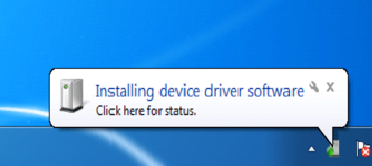
\includegraphics[width=10cm]{figures/5/1144124/Teori/1.png}
		\centering
        \label{1}
	\end{figure}
\item Karena Arduino Uno baru pertama kali terpasang, maka akan muncul pop up error seperti ini.
	\begin{figure}[H]
		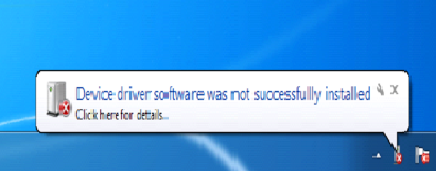
\includegraphics[width=10cm]{figures/5/1144124/Teori/2.png}
		\centering
	\end{figure}
\item Buka `Start' lalu cari Device Manager, kemudian klik `Device Manager'.
	\begin{figure}[H]
		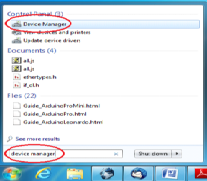
\includegraphics[width=5cm]{figures/5/1144124/Teori/3.png}
		\centering
	\end{figure}
\item Setelah Device Manager terbuka, silahkan cari `Unknown Device' yang berada di Other Device.
	\begin{figure}[H]
		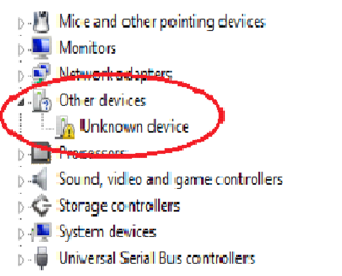
\includegraphics[width=5cm]{figures/5/1144124/Teori/4.png}
		\centering
	\end{figure}
\item Kemudian klik kanan pada `Unknown Device', lalu pilih `Update Driver Software'.
	\begin{figure}[H]
		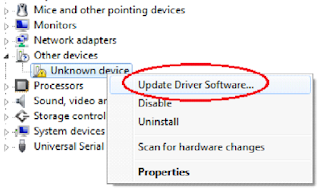
\includegraphics[width=7cm]{figures/5/1144124/Teori/5.png}
		\centering
	\end{figure}
\item Setelah itu muncul window baru, lalu pilih `Browse my computer for driver software'.
	\begin{figure}[H]
		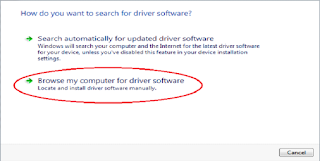
\includegraphics[width=7cm]{figures/5/1144124/Teori/6.png}
		\centering
	\end{figure}
\item Lalu cari folder yang terinstall Arduino IDE dengan mengklik browse. Kemudian klik `Next'.
	\begin{figure}[H]
		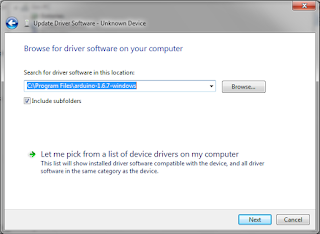
\includegraphics[width=7cm]{figures/5/1144124/Teori/7.png}
		\centering
	\end{figure}
\item Windows akan mencari dan menginstall driver yang berada pada folder tersebut.
	\begin{figure}[H]
		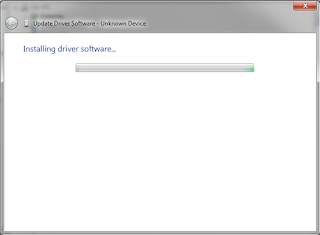
\includegraphics[width=7cm]{figures/5/1144124/Teori/8.png}
		\centering
	\end{figure}
\item Setelah itu akan muncul window, lalu klik `Install'.
	\begin{figure}[H]
		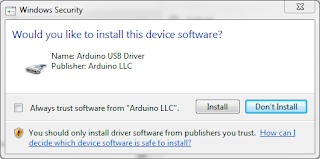
\includegraphics[width=5cm]{figures/5/1144124/Teori/9.png}
		\centering
	\end{figure}
\item Jika berhasil terinstal maka akan muncul window seperti ini.
	\begin{figure}[H]
		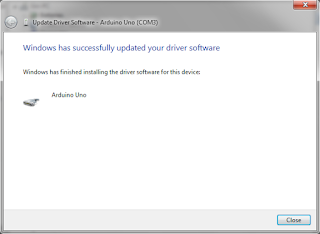
\includegraphics[width=5cm]{figures/5/1144124/Teori/10.png}
		\centering
	\end{figure}
\end{enumerate}

\subsection{Soal No. 3}
Jelaskan bagaimana cara membaca baudrate dan port dari komputer yang sudah terinstall driver!
\textbf{Membaca Baudrate dari Komputer}
\begin{enumerate}
	\item Pertama buka `Start'. Cari `Device Manager', lalu klik.
	\begin{figure}[H]
		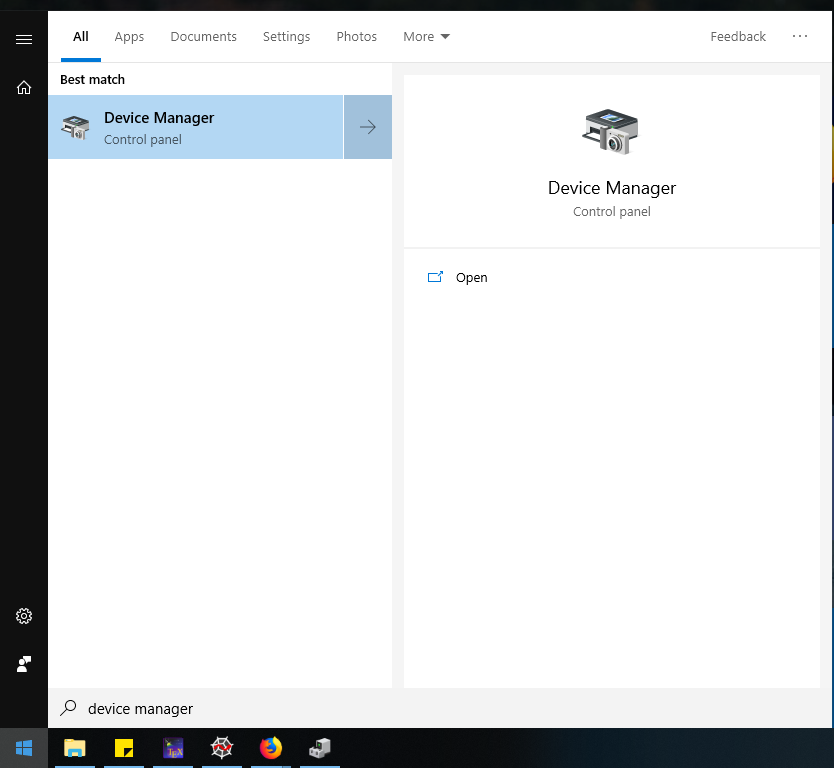
\includegraphics[width=5cm]{figures/5/1144124/Teori/d1.png}
		\centering
	\end{figure}
	\item Kemudian pilih `Ports (COM \& LPT)'.
	\begin{figure}[H]
		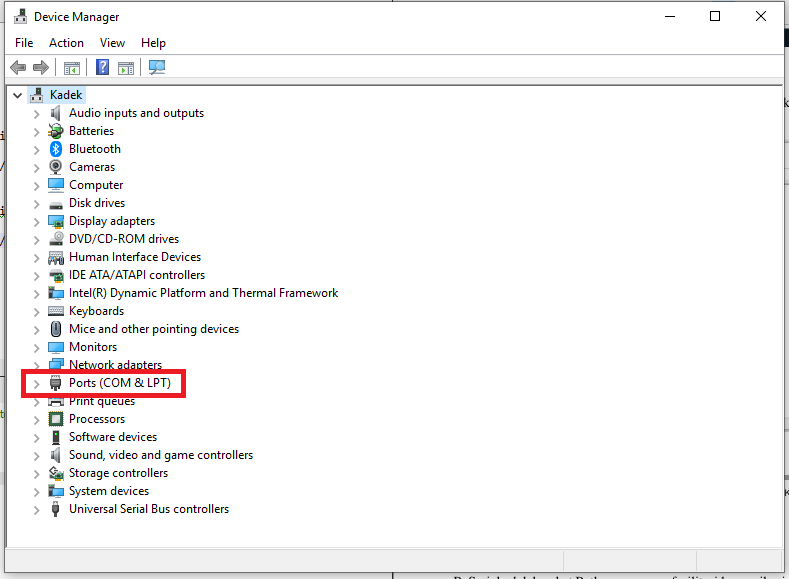
\includegraphics[width=5cm]{figures/5/1144124/Teori/d3.png}
		\centering
	\end{figure}
	\item Klik dua kali pada COM yang terhubung.
	\begin{figure}[H]
		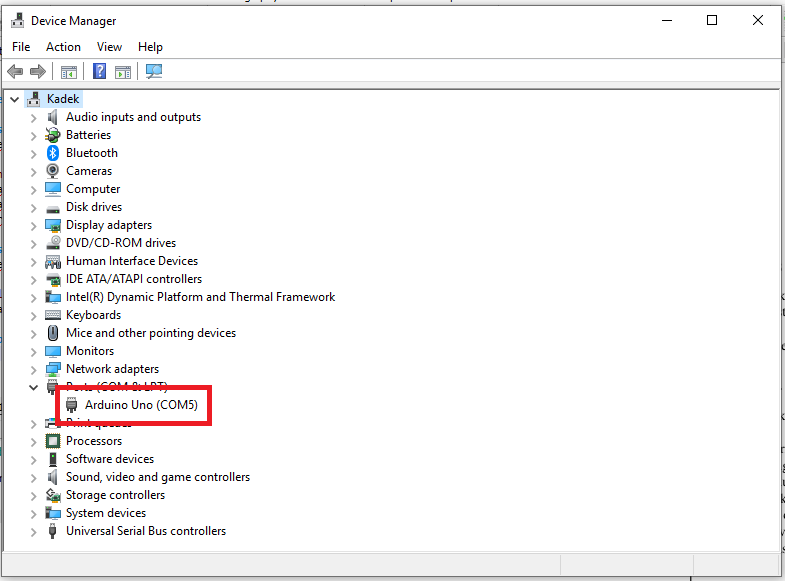
\includegraphics[width=5cm]{figures/5/1144124/Teori/d2.png}
		\centering
	\end{figure}
	\item Pilih tab `Port Settings', lalu lihat di `Bit per second'.
	\begin{figure}[H]
		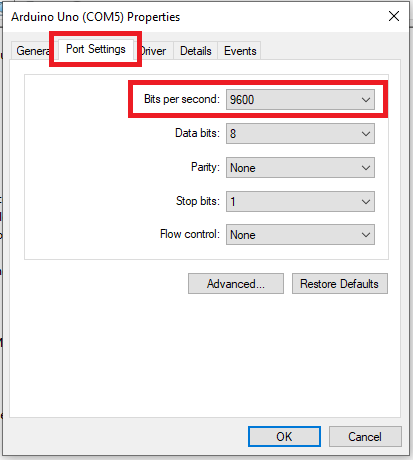
\includegraphics[width=5cm]{figures/5/1144124/Teori/d4.png}
		\centering
	\end{figure}
\end{enumerate}
\textbf{Membaca Port dari Komputer}
\begin{enumerate}
	\item Pertama buka `Start'. Cari `Device Manager', lalu klik.
	\begin{figure}[H]
		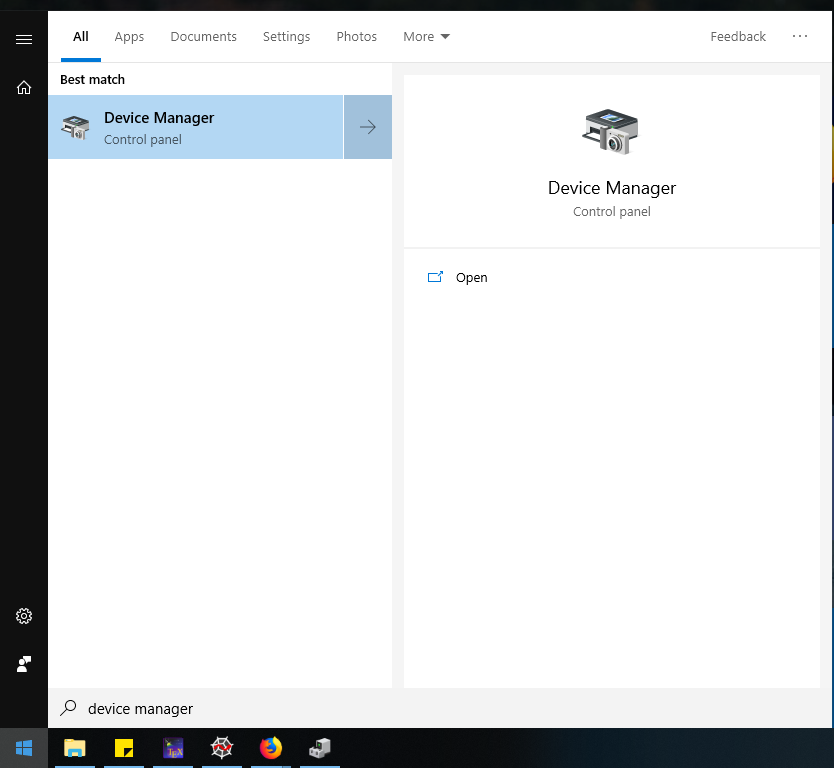
\includegraphics[width=5cm]{figures/5/1144124/Teori/d1.png}
		\centering
	\end{figure}
	\item Kemudian pilih `Ports (COM \& LPT)'.
	\begin{figure}[H]
		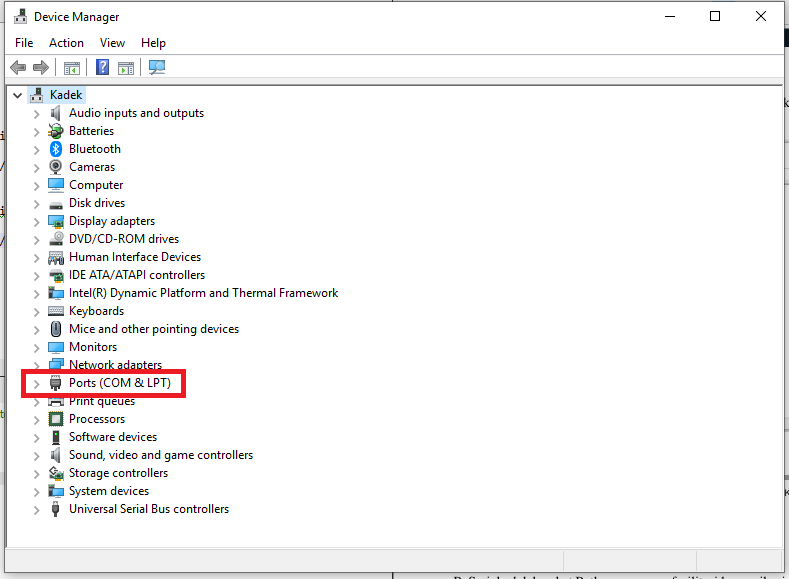
\includegraphics[width=5cm]{figures/5/1144124/Teori/d3.png}
		\centering
	\end{figure}
	\item Port dari Arduino telah terbaca oleh PC.
	\begin{figure}[H]
		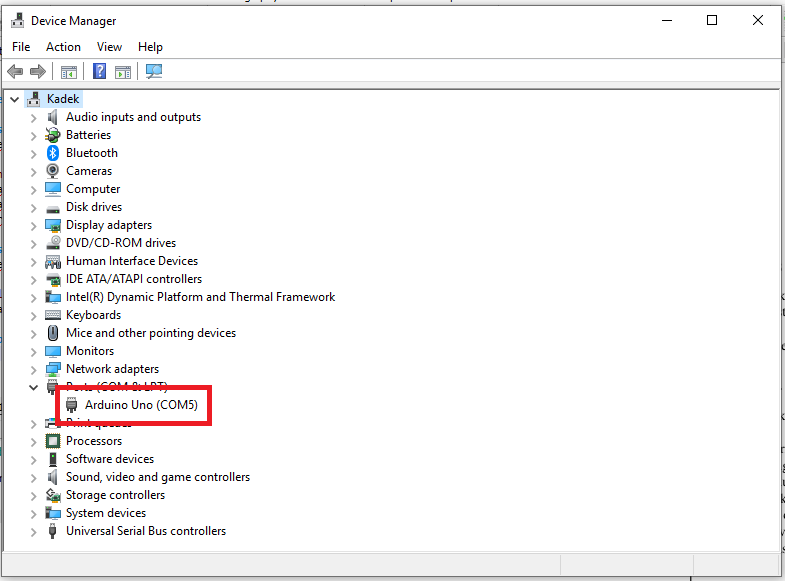
\includegraphics[width=5cm]{figures/5/1144124/Teori/d2.png}
		\centering
	\end{figure}
\end{enumerate}

\subsection{Soal No. 4}
Jelaskan sejarah library pyserial!

PySerial adalah paket Python yang memfasilitasi komunikasi serial antara PC dengan perangkat keras eksternal. PySerial menyediakan antarmuka untuk berkomunikasi melalui protokol komunikasi serial. Komunikasi serial adalah salah satu protokol komunikasi komputer tertua. Protokol komunikasi serial mendahului spesifikasi USB yang dapat digunakan oleh komputer dan perangkat keras lain seperti mouse, keyboard, dan webcam. USB adalah singkatan dari Universal Serial Bus. USB dibangun diatas dan memperluas antarmuka komunikasi serial asli.

\subsection{Soal No. 5}
Jelaskan fungsi-fungsi apa saja yang dipakai dari library pyserial!

Fungsi-fungsi yang dipakai dari library PySerial, yaitu:
\begin{enumerate}
	\item Serial - fungsi ini untuk membuka port serial.
	\item write(data) - fungsi ini menulis data lewat port serial.
	\item readline() - fungsi ini membaca sebuah string dari port serial.
	\item read(size) - fungsi ini untuk membaca jumlah byte dari port serial.
	\item close() - fungsi ini untuk menutup port serial.
\end{enumerate}

\subsection{Soal No. 6}
Jelaskan kenapa butuh perulangan dan tidak butuh perulangan dalam membaca serial!

Pada saat membaca serial di Arduino diperlukan perulangan agar bisa membaca data secara berulang kali sehingga data yang akan muncul banyak. Sedangkan apabila tidak membutuhkan perulangan maka Arduino hanya akan membaca data sekali saja.

\subsection{Soal No. 7}
Jelaskan bagaimana cara membuat fungsi yang mengunakan pyserial!
\lstinputlisting[caption = Fungsi yang menggunakan pyserial., firstline=1, lastline=7]{src/5/1144124/Teori/1144124.py}

\subsection{Praktek}
\subsubsection{Soal No. 1}
Buatlan fungsi (file terpisah/library dengan nama NPMrealtime.py) untuk mendapatkan data langsung dari arduino!

\lstinputlisting[caption = Fungsi untuk mendapatkan data dari Arduino., firstline=1, lastline=7]{src/5/1144124/Praktek/1144124realtime.py}

\subsubsection{Soal No. 2}
Buatlah fungsi (file terpisah/library dengan nama NPMsave.py) untuk mendapatkan data langsung dari ardduino dengan looping!
\lstinputlisting[caption = Fungsi untuk mendapatkan data langsung dari Arduino dengan looping., firstline=1, lastline=8]{src/5/1144124/Praktek/1144124save.py}

\subsubsection{Soal No. 3}
Buatlah fungsi (file terpisah/library dengan nama NPMrealtime.py) untuk mendapatkan data dari arduino dan langsung ditulis kedalam file csv!
\lstinputlisting[caption = Fungsi untuk mendapatkan data dari Arduino dan langsung ditulis kedalam file CSV., firstline=9, lastline=23]{src/5/1144124/Praktek/1144124realtime.py}

\begin{figure}[H]
	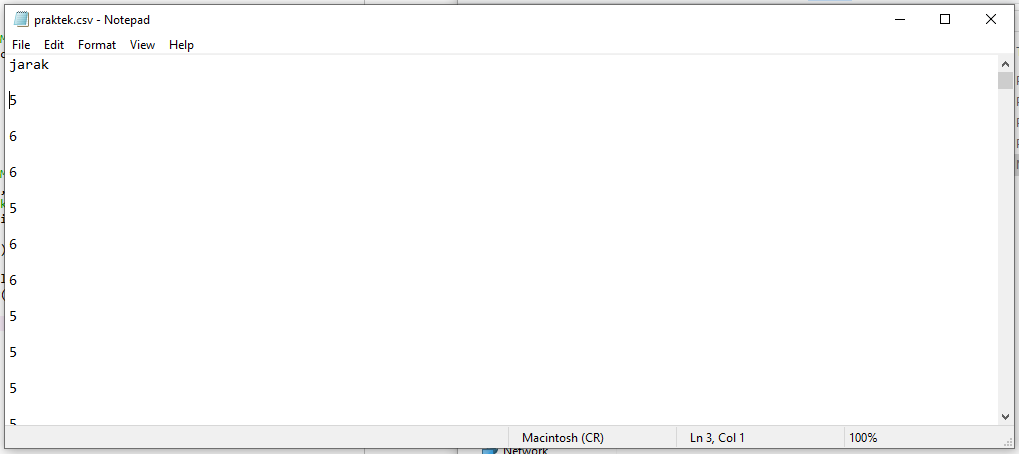
\includegraphics[width=12cm]{figures/5/1144124/Praktek/3.png}
	\centering
	\caption{Hasil dari pembacaan fungsi untuk mendapatkan data dari Arduino dan langsung ditulis kedalam file CSV.}
\end{figure}
\subsubsection{Soal No. 4}
Buatlah fungsi (file terpisah/library dengan nama NPMcsv.py) untuk membaca file csv hasil arduino dan mengembalikan ke fungsi!
\lstinputlisting[caption = Fungsi untuk membaca file CSV hasil Arduino dan mengembalikan fungsi., firstline=1, lastline=9]{src/5/1144124/Praktek/1144124csv.py}

\begin{figure}[H]
	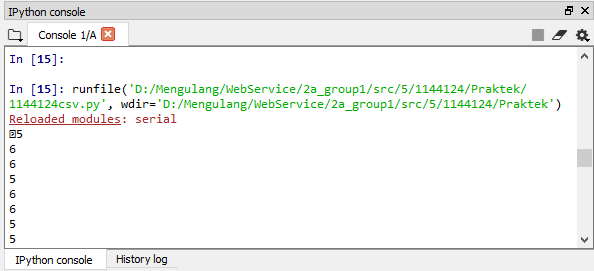
\includegraphics[width=12cm]{figures/5/1144124/Praktek/csv.png}
	\centering
	\caption{Hasil dari pembacaan fungsi untuk membaca file csv hasil arduino dan mengembalikan fungsi.}
\end{figure}
\subsubsection{Penanganan Error} 
\begin{itemize}
  \item Tuliskan peringatan error yang didapatkan dari mengerjakan prakter ketiga ini, dan jelaskan cara penanganan error tersebut. Dan buatlah satu fungsi yang menggunakan try except untuk menanggulangi error tersebut.
      Fungsi yang menggunakan try except untuk menanggulangi error.

\lstinputlisting[caption = Fungsi untuk menanggulangi error menggunakan Try Except., firstline=1, lastline=12]{src/5/1144124/Praktek/1144124.py}
\end{itemize}